\documentclass[t,14pt,aspectratio=169,usenames,dvipsnames,table]{beamer}
%%%%%%%%%%%%%%%%%%%%%%%%%%%%%%%%%%%%%%%%%%%%%%%%%%%%%%%%%%%%%%%%%%%%%%%%%%%%%%%%%%%%%%%
% To Pass graphics paths
%%%%%%%%%%%%%%%%%%%%%%%%%%%%%%%%%%%%%%%%%%%%%%%%%%%%%%%%%%%%%%%%%%%%%%%%%%%%%%%%%%%%%%%

\graphicspath{{./Figures/}}
\graphicspath{{./Figures/chapter-01/}}
%%%%%%%%%%%%%%%%%%%%%%%%%%%%%%%%%%%%%%%%%%%%%%%%%%%%%%%%%%%%%%%%%%%%%%%%%%%%%%%%%%%%%%%
% Packages Definition
%%%%%%%%%%%%%%%%%%%%%%%%%%%%%%%%%%%%%%%%%%%%%%%%%%%%%%%%%%%%%%%%%%%%%%%%%%%%%%%%%%%%%%%
%\input{preamble/ch_01_theme}
%\usepackage{preamble/dbt}
\usetheme[showmaxslides]{pureminimalistic}
%\usetheme[darkmode, showmaxslides]{pureminimalistic}





\newcommand{\code}[1]{\mbox{\color{yellow}{\texttt{\textbf{\normalsize #1}}}}}
\usepackage[toc,page]{appendix}
\usepackage{listings}
\usepackage{hyperref}
\usepackage{pgf,pgfpages}
\usepackage{graphicx}
\usepackage{units}
\usepackage[utf8]{inputenc}
\usepackage{multicol}
\usepackage{xspace}
\usepackage[utf8]{inputenc}
\usepackage{textcomp}% for '\textdegree' macro
\usepackage{utopia} %font utopia imported
\usepackage{fontawesome5}
\usepackage[center]{caption}
\usepackage{subcaption}
\usepackage{gensymb}
\usepackage{adjustbox}
\usepackage{marginnote}
\usepackage{makecell}
\usepackage{textpos}
\usepackage[default]{lato}
\usepackage[font=small,skip=0pt]{caption}
\usepackage{xcolor,colortbl}
\usepackage{import}
\usepackage{marvosym}
\usepackage{ulem} %Strikethrough
\usepackage[inkscapelatex=false]{svg}


%\overfullrule=2cm
%%%%%%%%%%%%%%%%%%%%%%%%%%%%%%%%%%%%%%%%%%%%%%%%%%%%%%%%%%%%%%%%%%%%%%%%%%%%%%%%%%%%%%%
\input{preamble/preamble_quote_custom_commands.tex}
%%%%%%%%%%%%%%%%%%%%%%%%%%%%%%%%%%%%%%%%%%%%%%%%%%%%%%%%%%%%%%%%%%%%%%%%%%%%%%%%%%%%%%%
\input{preamble/preamble_custom_commands.tex}
%%%%%%%%%%%%%%%%%%%%%%%%%%%%%%%%%%%%%%%%%%%%%%%%%%%%%%%%%%%%%%%%%%%%%%%%%%%%%%%%%%%%%%%
\input{preamble/tikz_preamble.tex}
%%%%%%%%%%%%%%%%%%%%%%%%%%%%%%%%%%%%%%%%%%%%%%%%%%%%%%%%%%%%%%%%%%%%%%%%%%%%%%%%%%%%%%%
%%%%%%%%%%%%%%%%%%%%%%%%%%%%%%%%%%%%%%%%%%%%%%%%%%%%%%%%%%%%%%%%%%%%%%%%%%%%%%%%%%%%%%%% 
%To define Code Syntax Scala
%%%%%%%%%%%%%%%%%%%%%%%%%%%%%%%%%%%%%%%%%%%%%%%%%%%%%%%%%%%%%%%%%%%%%%%%%%%%%%%%%%%%%%%% 
% Scala
%%%%%%%%%%%%%%%%%%%%%%%%%%%%%%%%%%%%%%%%%%%%%%%%%%%%%%%%%%%%%%%%%%%%%%%%%%%%%%%%%%%%%%%% 
\definecolor{mymauve}{rgb}{0.58,0,0.82}
\definecolor{dkgreen}{rgb}{0,0.6,0}
\definecolor{ltgray}{rgb}{0.5,0.5,0.5}
\usepackage{caption} % Add the caption package

% Redefine the lstlisting format to remove the unwanted prefix
\DeclareCaptionFormat{mylst}{#1#2#3}
\DeclareCaptionFont{mycolor}{\color{red}}
\renewcommand\lstlistingname{Code Snippet:}
\renewcommand\lstlistlistingname{Code Snippet:}
%\DeclareCaptionStyle{listing} [justification=raggedright,indention=0pt, labelfont=bf]{}
%\captionsetup[lstlisting]{style=listing, labelsep=none}

\captionsetup[lstlisting]{format=mylst,labelfont={color=harvardcrimson},labelsep=space,justification=raggedright}

\lstset{%
	frame=tb,
	language=scala,
	aboveskip=3mm,
	belowskip=3mm,
	showstringspaces=false,
	columns=flexible,
	numbers=left,                   % where to put the line-numbers
	numberstyle=\tiny\color{gray},  % the style that is used for the line-numbers
	stepnumber=1,                   % the step between two line-numbers. If it's 1, each line will be numbered
	numbersep=5pt,                  % how far the line-numbers are from the code
	backgroundcolor=\color{white},  % choose the background color. You must add 
	keywordstyle=\color{blue},
	commentstyle=\color{dkgreen},
	%  stringstyle=\color{mauve},
	stringstyle=\color{myorange},
	frame=single,
	breaklines=true,
	breakatwhitespace=true,
	breakindent=20pt,
	tabsize=4,
	frameround=tttt,
	escapeinside={\%*}{*)},        % to add a comment within your code
	emph={count,take,textFile,filter,first,collect,mkString}, % Scala functions
	emphstyle={\color{mauve}},
	morekeywords ={val,sc},        % to add more keywords to the set  
	showspaces=false,
	showstringspaces=false,
	keepspaces=true
}

%%%%%%%%%%%%%%%%%%%%%%%%%%%%%%%%%%%%%%%%%%%%%%%%%%%%%%%%%%%%%%%%%%%%%%%%%%%%%%%%%%%%%%%% 
\lstset{%
	language=SQL,
	backgroundcolor=\color{white},
	basicstyle=\footnotesize,
	%breakatwhitespace=false,
	breaklines=true,
	captionpos=b,
	numbers=left,                   % where to put the line-numbers
	numberstyle=\tiny\color{gray},  % the style that is used for the line-numbers
	stepnumber=1,                   % the step between two line-numbers. If it's 1, each line will be numbered
	numbersep=5pt,                  % how far the line-numbers are from the code
	commentstyle=\color{dkgreen},
	%deletekeywords={...},
	%escapeinside={\%*}{*)},
	%extendedchars=true,
	frame=tb,
	keepspaces=false,
	keywordstyle=\color{blue},
	morekeywords={modify,MODIFY,ALL, ALTER, AND, ARRAY, AS, AUTHORIZATION, BETWEEN, BIGINT, BINARY, BOOLEAN, BOTH, BY, CASE, CAST, CHAR, COLUMN, CONF, CREATE, CROSS, CUBE, CURRENT, CURRENT_DATE, CURRENT_TIMESTAMP, CURSOR, DATABASE, DATE, DECIMAL, DELETE, DESCRIBE, DISTINCT, DOUBLE, DROP, ELSE, END, EXCHANGE, EXISTS, EXTENDED, EXTERNAL, FALSE, FETCH, FLOAT, FOLLOWING, FOR, FROM, FULL, FUNCTION, GRANT, GROUP, GROUPING, HAVING, IF, IMPORT, IN, INNER, INSERT, INT, INTERSECT, INTERVAL, INTO, IS, JOIN, LATERAL, LEFT, LESS, LIKE, LOCAL, MACRO, MAP, MORE, NONE, NOT, NULL, OF, ON, OR, ORDER, OUT, OUTER, OVER, PARTIALSCAN,PARTITIONED, STORED, TERMINATED, ROW, FORMAT, PARTITION,PERCENT, PRECEDING, PRESERVE, PROCEDURE, RANGE, READS, REDUCE, REVOKE, RIGHT, ROLLUP, ROW, ROWS, SELECT, SET, SMALLINT, TABLE, TABLESAMPLE, THEN, TIMESTAMP, TO, TRANSFORM, TRIGGER, TRUE, TRUNCATE, UNBOUNDED, UNION, UNIQUEJOIN, UPDATE, USER, USING, UTC_TMESTAMP, VALUES, VARCHAR, WHEN, WHERE, WINDOW, WITH, BY},
	numbers=left,
	numbersep=15pt,
	numberstyle=\tiny,
	rulecolor=\color{ltgray},
	showstringspaces=false,
	showtabs=false,
	stepnumber=1,
	tab=2,
	literate={\ \ }{{\ }}1,
	keepspaces=true,
	showtabs=false,
	caption=Example SQL Query,
	showspaces=false,
	xleftmargin=4.0ex,	
	keepspaces=true
}
%%%%%%%%%%YML 
\lstdefinestyle{yaml}{
    basicstyle=\ttfamily\small,
    breaklines=true,
    frame=single,
	morekeywords={Name, Type, Operations, Condition,TableName},
    keywordstyle=\color{blue},
    morestring=[b]",
    stringstyle=\color{red},
    keepspaces=true
}

\lstdefinelanguage{my-yaml}{
  keywords={spec, containers, name,Type,TableName,PruningEnabled,PruningEnabled,RelevantBuckets,Condition}, % ,... all the keyword you want
  keywordstyle=\color{blue}\bfseries,
  moredelim=[is][commentstyle]{||}{££}, % invisible custom delimiters
  identifierstyle=\color{black},
  sensitive=false,
  comment=[l]{\#},
  commentstyle=\color{olive}\ttfamily,
  stringstyle=\color{orange}\ttfamily,
  morestring=[b]',
  morestring=[b]"
}
\lstdefinestyle{my-yamll}{	
     basicstyle=\color{black}\footnotesize,
     rulecolor=\color{blue},
     string=[s]{'}{'},
     stringstyle=\color{black},
     comment=[l]{:},
     commentstyle=\color{blue},
     morecomment=[l]{-}
 }
%%%%%%%%%%%%%%%%%%%%%%%%%%%%%%%%%%%%%%%%%%%%%%%%%%%%%%%%%%%%%%%%%%%%%%%%%%%

\newcommand\JSONnumbervaluestyle{\color{red}}
\newcommand\JSONstringvaluestyle{\color{red}}

% switch used as state variable
\newif\ifcolonfoundonthisline

\makeatletter

\lstdefinestyle{json}
{
	showstringspaces    = false,
	keywords            = {false,true},
alsoletter          = 0123456789.,
morestring          = [s]{"}{"},
framextopmargin=3pt,
stringstyle         = \ifcolonfoundonthisline\JSONstringvaluestyle\fi,
MoreSelectCharTable =%
	\lst@DefSaveDef{`:}\colon@json{\processColon@json},
basicstyle          = \ttfamily,
keywordstyle        = \ttfamily\bfseries,
}

% flip the switch if a colon is found in Pmode
\newcommand\processColon@json{%
	\colon@json%
	\ifnum\lst@mode=\lst@Pmode%
	\global\colonfoundonthislinetrue%
	\fi
}

\lst@AddToHook{Output}{%
	\ifcolonfoundonthisline%
	\ifnum\lst@mode=\lst@Pmode%
	\def\lst@thestyle{\JSONnumbervaluestyle}%
	\fi
	\fi
%override by keyword style if a keyword is detected!
	\lsthk@DetectKeywords% 
}

% reset the switch at the end of line
\lst@AddToHook{EOL}%
{\global\colonfoundonthislinefalse}
%%%%%%%%%%%%%%%%%%%%%%%%%%%%%%%%%%%%%%%%%

%%%%%%%%%%%%%%%%%%%%%%%%%%%%%%%%%%%%%%%%%%%%%%%%%%%%%%%%%%%%%%%%%%%%%%%%%%%
%%% Local Variables:
%%% mode: latex
%%% TeX-master: "../main"
% !TeX root = ../main.tex
%%% TeX-engine: xetex
%%% End:
%%%%%%%%%%%%%%%%%%%%%%%%%%%%%%%%%%%%%%%%%%%%%%%%%%%%%%%%%%%%%%%%%%%%%%%%%%%%%%%%%%%%%%%
\usepackage{tikz,lipsum,fontspec}
\usetikzlibrary{shapes.callouts,decorations.pathmorphing}
\newfontfamily\comic{Comic Sans MS}
%update for publishing
\setbeamersize{text margin left=5pt,text margin right=3.5cm}
%\setbeamersize{text margin left=5pt}

%%remove logo for publishing
%\logo{%
%	\includegraphics[width=4cm,height=3.5cm]{./Figures/chapter-00/logos.png}%
%}'\mode<presentation> {




\AtBeginDocument{
  \catcode`_=12
  \begingroup\lccode`~=`_
  \lowercase{\endgroup\let~}\sb
  \mathcode`_="8000
}
\setbeamercolor{caption name}{fg=orange}
\setlength{\belowcaptionskip}{10pt}

\setbeamertemplate{itemize/enumerate body begin}{\small}
%\setbeamertemplate{navigation symbols}{}
%%%%%%%%%%%%%%%%%%%%%%%%%%%%%%%%%%%%%%%%%%%%%%%%%%%%%%%%%%%%%%%%%%%%%%%%%%%%%%%%%%%%%%%
%\addtobeamertemplate{frametitle}{}{\vspace{-0.3 cm}}
%%%%%%%%%%%%%%%%%%%%%%%%%%%%%%%%%%%%%%%%%%%%%%%%%%%%%%%%%%%%%%%%%%%%%%%%%%%%%%%%%%%%%%%
%%% Local Variables:
%%% mode: latex
%%% TeX-master: "../main"
% !TeX root = ../main.tex
%%% TeX-engine: xetex
%%% End:

%This block of code defines the information to appear in the
%Title page
\title[Data Engineering In Depth] %optional
{(Big) Data Engineering In Depth}

%\subtitle{From Beginner to Professional}


\author[Moustafa Mahmoud] {
	Moustafa Mahmoud \newline 	
	\footnotesize \textcolor{ballblue}{\textbf{Data Solution Architect}} \newline
}

\date[\today] % (optional)
{The Definitive Guide to Big Data Engineering Tasks}

%\logo{\includegraphics[height=1.5cm]{lion-logo.png}}

%End of title page configuration block
%------------------------------------------------------------

%%%%%%%%%%%%%%%%%%%%%%%%%%%%%%%%%%%%%%%%%%%%%%%%%%%%%%%%%%%%%%%%%%%%%%%%%%%
%%% Local Variables:
%%% mode: latex
%%% TeX-master: "../main"
%%% TeX-engine: xetex
%%% End:

\renewcommand{\logotitle}{\includegraphics%
	[width=.2\linewidth]{logos/header_logo.png}}
\renewcommand{\logoheader}{\includegraphics%
	[width=0\linewidth]{logos/header_logo.png}}
\renewcommand{\logofooter}{\includegraphics%
	[width=.15\linewidth]{logos/header_logo.png}}
\date{\today}

%------------------------------------------------------------
\begin{document}
    %---------------------------------------------------------
    %The next statement creates the title page.
    \frame{\titlepage}
    %---------------------------------------------------------
    %%TOC
	%\begin{frame}[allowframebreaks]
	%\frametitle{Table of Contents}
	%\tableofcontents
	%\end{frame}
    %---------------------------------------------------------
    %%%%%%%%%%%%%%%%%%%%%%%%%%%%%%%%%%%%%%%%%%%%%%%%%%%%%%%%%%%%%%%%%%%%%%%%%%%%%%%%%%%%%%%
%    \include{Ch00-CourseOverview/CourseOverview.tex}
%    \include{Ch01-Introduction-data-management/Ch01-Introduction-data-management}
%     %\section{Introduction To Distributed Systems}
%\input{Ch02-Introduction-To-Distributed-Systems/Ch01-01-sub-intro}
%%%%%%%%%%%%%%%%%%%%%%%%%%%%%%%%%%%%%%%%%%%%%%%%%%%%%%\\
%\input{Ch02-Introduction-To-Distributed-Systems/Ch01-02-sub-intro}
%%%%%%%%%%%%%%%%%%%%%%%%%%%%%%%%%%%%%%%%%%%%%%%%%%%%%%\\



%%%%%%%%%%%%%%%%%%%%%%%%%%%%%%%%%%%%%%%%%%%%%%%%%%%%%%%
\begin{frame}[c]{ }
	\centering     
	
	\textcolor{offgreen}{ \large Previous video recap!}
\end{frame}

%\input{Ch02-Introduction-To-Distributed-Systems/Ch01-03-sub-hadoop-intro}

%\input{Ch02-Introduction-To-Distributed-Systems/Ch01-03-sub-hdfs-intro}

%\input{Ch02-Introduction-To-Distributed-Systems/Ch01-03-sub-yarn-intro}

%
%%%%%%%%%%%%%%%%%%%%%%%%%%%%%%%%%%%%%%%%%%%%%%%%%%%%%%
\begin{frame}[c]{ }
	\frametitle{Hadoop Core Concepts }
	
	
	\begin{itemize}  [<+->]
		\item [--] HDFS.
		\item [--] YARN.
		\item [--] Map-Reduce.
		
	\end{itemize}
\end{frame}
%%%%%%%%%%%%%%%%%%%%%%%%%%%%%%%%%%%%%%%%%%%%%%%%%%%%%%
\begin{frame}[c]{ }
	\frametitle{ Hadoop Map Reduce}
	\centering     
	
	\textcolor{offgreen}{ \large Introduction To Hadoop Map Reduce API}
\end{frame}
%%%%%%%%%%%%%%%%%%%%%%%%%%%%%%%%%%%%%%%%%%%%%%%%%%%%%%	

\begin{frame}
\frametitle{The basic idea of MapReduce}
We break this into three stages
\begin{itemize}  [<+->]
	\item Map.
	\item Shuffle/Group (Mapper Intermediates).
	\item Reduce			
\end{itemize}
\footnotetext[1]{This example taken from  \href{https://reberhardt.com/cs110/summer-2018/lecture-notes/lecture-14/}{https://reberhardt.com/cs110/summer-2018/lecture-notes/lecture-14/}	} 
\end{frame}
%%%%%%%%%%%%%%%%%%%%%%%%%%%%%%%%%%%%%%%%%%%%%%%%%%%%%%
\begin{frame}
\frametitle{Map}
We distribute our raw ingredients amongst the workers.
\begin{figure}
	\includegraphics[width=.5\textwidth,height=.7\textheight]{./Figures/chapter-02/map-reduce-map-side.jpeg}
\end{figure}			
\footnotetext[1]{{\tiny This example taken from  \href{https://reberhardt.com/cs110/summer-2018/lecture-notes/lecture-14/}{https://reberhardt.com/cs110/summer-2018/lecture-notes/lecture-14/}	} }
\end{frame}
%%%%%%%%%%%%%%%%%%%%%%%%%%%%%%%%%%%%%%%%%%%%%%%%%%%%%%
\begin{frame}
\frametitle{Shuffle/Group}
We will organise and group the processed ingredients into piles, so that making a sandwich becomes easy.
\begin{figure}
	\includegraphics[width=.7\textwidth,height=.64\textheight]{./Figures/chapter-02/map-reduce-shuffle.png}
\end{figure}			
\footnotetext[1]{{\tiny This example taken from  \href{https://reberhardt.com/cs110/summer-2018/lecture-notes/lecture-14/}{https://reberhardt.com/cs110/summer-2018/lecture-notes/lecture-14/}	}} 
\end{frame}
%%%%%%%%%%%%%%%%%%%%%%%%%%%%%%%%%%%%%%%%%%%%%%%%%%%%%%
\begin{frame}
\frametitle{Reduce}
we’ll combine the ingredients into a sandwich
\begin{figure}
	\includegraphics[width=.96\textwidth,height=.7\textheight]{./Figures/chapter-02/map-reduce-reduce-side.png}
\end{figure}			
\footnotetext[1]{ {\tiny This example taken from  \href{https://reberhardt.com/cs110/summer-2018/lecture-notes/lecture-14/}{https://reberhardt.com/cs110/summer-2018/lecture-notes/lecture-14/}	}} 
\end{frame}
%%%%%%%%%%%%%%%%%%%%%%%%%%%%%%%%%%%%%%%%%%%%%%%%%%%%%%
\begin{frame}[plain,c]
	\frametitle{Case Study Example 1}
	\begin{figure}
		\centering
		\input{./Figures/chapter-02/ds_case_study_1_1.tex}
		\caption{Convert text to upper text, for example, The -> THE } \label{fig:DS3}
	\end{figure}
	
\end{frame}
%%%%%%%%%%%%%%%%%%%%%%%%%%%%%%%%%%%%%%%%%%%%%%%%%%%%%%
\begin{frame}[plain,c]
	\frametitle{Case Study Example 1}
	\begin{figure}
		\centering
		\input{./Figures/chapter-02/ds_case_study_1_3.tex}
	\end{figure}


\end{frame}

%%%%%%%%%%%%%%%%%%%%%%%%%%%%%%%%%%%%%%%%%%%%%%%%%%%%%%
\begin{frame}[plain,c]
	\frametitle{Case Study Example 2}
	\begin{figure}
		\centering
		\input{./Figures/chapter-02/ds_case_study_2_1.tex}
	\end{figure}
	
\end{frame}

%%%%%%%%%%%%%%%%%%%%%%%%%%%%%%%%%%%%%%%%%%%%%%%%%%%%%%
\begin{frame}

	\begin{figure}
		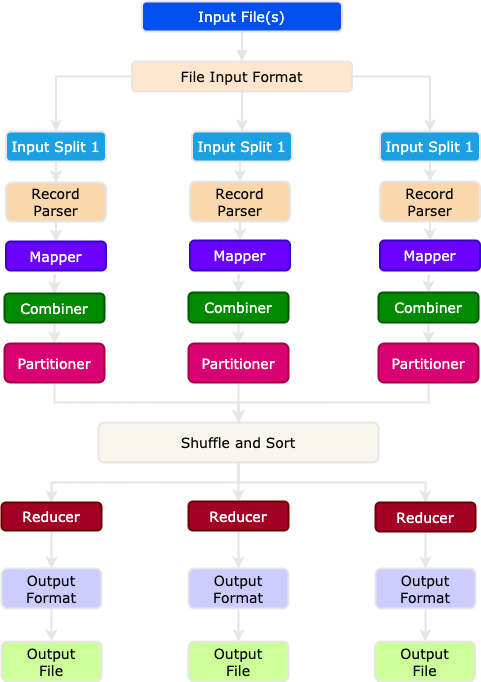
\includegraphics[height=.925\textheight]{./Figures/chapter-02/Map-Reduce.png}
				\caption{Map Reduce Stages } \label{fig:MRSteps}
	\end{figure}			
\end{frame}
%%%%%%%%%%%%%%%%%%%%%%%%%%%%%%%%%%%%%%%%%%%%%%%%%%%%%%
\begin{frame}
	
	\begin{figure}
		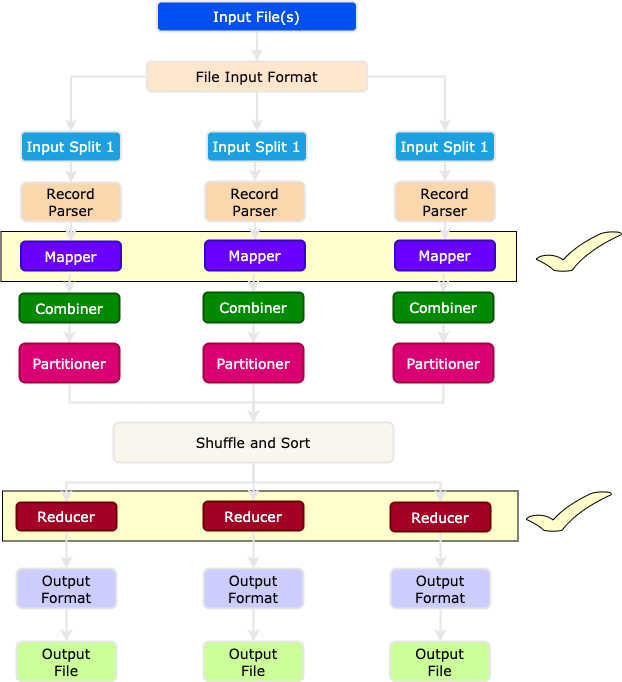
\includegraphics[height=.925\textheight]{./Figures/chapter-02/Map-Reduce_2.png}
		\caption{Map Reduce Stages } \label{fig:MRSteps2}
	\end{figure}			
\end{frame}
%%%%%%%%%%%%%%%%%%%%%%%%%%%%%%%%%%%%%%%%%%%%%%%%%%%%%%
\begin{frame}[c]{ }
	\frametitle{Map Reduce (word count) Deep Dive }
	
	The Map-Reduce consists of three "main" parts
	
	\begin{itemize}  [<+->]
		\item [--] The Driver.
		\item [--] The Mapper.
		\item [--] The Reducer.
		
	\end{itemize}
\end{frame}
%%%%%%%%%%%%%%%%%%%%%%%%%%%%%%%%%%%%%%%%%%%%%%%%%%%%%%
\begin{frame}[c]{ }
	\frametitle{ Hadoop Map Reduce API}
	\centering     
	
	\textcolor{offgreen}{ \large Hadoop Map Reduce API Deep Dive}
\end{frame}
%%%%%%%%%%%%%%%%%%%%%%%%%%%%%%%%%%%%%%%%%%%%%%%%%%%%%%
\begin{frame}[c]{ }
	\frametitle{The Driver }

	\begin{itemize}  [<+->]
		\item [--] The code that runs on the client machine configures the job details by creating an object from the \code{Job}  class, which implements the \code{JobContext} interface.
		\item [--] It submits the job to the cluster.		
		\item [--] It parses job arguments to identify job parameters, for example, input/output directories.. 
		
	\end{itemize}

\end{frame}
%%%%%%%%%%%%%%%%%%%%%%%%%%%%%%%%%%%%%%%%%%%%%%%%%%%%%%
\begin{frame}[c]{ }
	\frametitle{The Driver:  Job Configuration}
	

The \code{Job}  object allows you to set configuration for your \code{Map-Reduce} job:
			\begin{itemize}  [<+->]
				\item [--] You can configure the \code{Mapper} \& the \code{Reducer} classes.
				\item [--] Set the \code{Mapper} input/output key \& value data types.
				\item [--] Set the \code{Reducer} input/output key \& value data types.
	
		
			\end{itemize}		

	
\end{frame}
%%%%%%%%%%%%%%%%%%%%%%%%%%%%%%%%%%%%%%%%%%%%%%%%%%%%%%
\begin{frame}[c]{ }
	\frametitle{The Driver:  Job Configuration}
	
	\begin{itemize}  [<+->]
		\item [--] We can configure file input directory and output.
		\item [--] We configure the output path using \code{FileOutputFormat.setOutputPath()} to specify the reducers' directory to write the output data.
	\end{itemize}		
	
\end{frame}
%%%%%%%%%%%%%%%%%%%%%%%%%%%%%%%%%%%%%%%%%%%%%%%%%%%%%%
\begin{frame}[c]{ }
	\frametitle{The Driver:  Job Configuration}
	
	\begin{itemize}  [<+->]
		\item [--] We configure the input path using \code{FileInputFormat.setInputPaths()}, and by default, it will read all the files in the specified directories and send them to the mappers.
		
		\item [--] We can use \code{Hadoop glob patterns} to read directory patterns, for example, \textit{/warehouse/public/sales*}.
		\item [--] We can call \code{FileInputFormat.addInputPath()} to multiple times by specifying a single file or directory. 
		
	\end{itemize}		
	
	\footnotetext[1]{For more details, please read HTDG. Ch.3 File patterns and PathFilter sections.	} 
\end{frame}
%%%%%%%%%%%%%%%%%%%%%%%%%%%%%%%%%%%%%%%%%%%%%%%%%%%%%%
\begin{frame}[c]{ }
	\frametitle{ Hadoop Map Reduce API}
	\centering     
	
	\textcolor{offgreen}{ \large Please read HTDG. Ch.3 The Java Interface}
\end{frame}
%%%%%%%%%%%%%%%%%%%%%%%%%%%%%%%%%%%%%%%%%%%%%%%%%%%%%%


\begin{frame}[c]{ }
	\frametitle{The Driver:  Job Configuration }
	
		
		\begin{itemize}  [<+->]

			\item [--] You could set driver configurations globally using Hadoop configurations.
			\item [--] Any options not specified in the job configuration will use the Hadoop default values.
			\item [--] We use the \code{Job} object to specify the job name and check its state..
		
			
	\end{itemize}
	
\end{frame}
%%%%%%%%%%%%%%%%%%%%%%%%%%%%%%%%%%%%%%%%%%%%%%%%%%%%%%
\begin{frame}[c]{ }
	\frametitle{The Driver:  Job Configuration }
	

	\begin{itemize}  [<+->]
		
	\item [--] It is optional to set the mapper and reducer classes.
	\item [--] Hadoop uses its default \code{IdentityMapper} and \code{IdentityReducer}.		
		
	\end{itemize}
	
\end{frame}
%%%%%%%%%%%%%%%%%%%%%%%%%%%%%%%%%%%%%%%%%%%%%%%%%%%%%%
\begin{frame}[c]{ }
	\frametitle{The Driver:  Job Configuration }
	
	
	Lunch a Map-Reduce job:
	\begin{itemize}  [<+->]
		
		\item [--] The \code{waitForCompletion()} method in the \code{Job} class launches the job and polls for progress. In addition, it writes the logs and summarizing the Map-Reduce job progress and changes.

	\item [--] When the job completes successfully, the job counters are displayed. Otherwise, the error that caused the job to fail is logged to the console.
		
	\end{itemize}
	
\end{frame}
%%%%%%%%%%%%%%%%%%%%%%%%%%%%%%%%%%%%%%%%%%%%%%%%%%%%%%
\begin{frame}[c]{ }
	\frametitle{InputFormat}
	
	\begin{itemize}  [<+->]
		\item [--] TheThe driver defines the \code{InputFormat}; then the \code{InputFormat} creates a \code{RecordReader"} object that parses the input data into key/value pairs passed to the mapper.
		\item [--] For example: \code{TextInputFormat}:
		\begin{itemize}  [<+->]
			
			\item It is the default.
			\item It creates \code{LineRecordReader} objects.
			\item Key: is the line offest in the file.
			\item Value: is the line which terminated by "\textbackslash n".
		\end{itemize}		
		
		
	\end{itemize}		
	
\end{frame}
%%%%%%%%%%%%%%%%%%%%%%%%%%%%%%%%%%%%%%%%%%%%%%%%%%%%%%
\begin{frame}[c]{ }
	\frametitle{Keys and Values}
	
	\begin{itemize}  [<+->]
		\item [--] Keys and Values in Hadoop are java \code{Objects} not \code{Java primitives types}.
		\item [--] Values are objects which implement \code{Writable}.
		\item [--] Keys are objects which implement \code{WritableComparable}.

		
	\end{itemize}		
	
\end{frame}
%%%%%%%%%%%%%%%%%%%%%%%%%%%%%%%%%%%%%%%%%%%%%%%%%%%%%%
\begin{frame}[c]{ }
	\frametitle{What is Writable?}
	
	\begin{itemize}  [<+->]
		\item [--] \code{Writable} is an interface in Hadoop.
		\item [--] \code{Writables} are used for data type "serialization" in Hadoop to translate/serialize "primitive java data types" to "Hadoop data types", Ex: int to IntWritable and String to Text.
		\item [--] Hadoop uses the \code{Writable} interface for data transfer in the cluster and network.
		
		
	\end{itemize}		
	
\end{frame}
%%%%%%%%%%%%%%%%%%%%%%%%%%%%%%%%%%%%%%%%%%%%%%%%%%%%%%
\begin{frame}[c]{ }
	\frametitle{What is WritableComparable?}
	
	\begin{itemize}  [<+->]
		\item [--] A \code{WritableComparable} is a \code{Writable} which is also \code{Comparable}.
		\item [--] We can compare two \code{WritableComparables} against each other to determine their \textbf{\underline{\textit{order}}}, for example, we could need to compare the order of two Text "Apple vs. Cat or numbers ordering" to understand the ordering mechanism. 
		\item [--] Obviously, the reason we have Keys to be \code{WritableComparable} is that they are passed to the reducer in \underline{\textit{\textbf{sorted order}}}.
		\item [--] Note: All Hadoop implemented types are both \code{Writable} and \code{WritableComparable}.
		
		
	\end{itemize}		
	
\end{frame}
%%%%%%%%%%%%%%%%%%%%%%%%%%%%%%%%%%%%%%%%%%%%%%%%%%%%%%
\begin{frame}[c]{ }
	\frametitle{Map Reduce (word count) Deep Dive }
	
	The Map-Reduce example consists of three main parts
	
	\begin{itemize}  [<+->]
		\item [--] \sout{The Driver}.
		\item [--] The Mapper.

		
	\end{itemize}
\end{frame}
%%%%%%%%%%%%%%%%%%%%%%%%%%%%%%%%%%%%%%%%%%%%%%%%%%%%%%
\begin{frame}[c]{ }
	\frametitle{The Mapper}
		
	\begin{itemize}  [<+->]
		
		\item [--] The mapper class deals with a single input split.
		
		\item [--] All mapper classes must extend the \code{Mapper} base class.

		\item [--] All mapper must specify the key and values for input and output.		
		
		\item [--] All mappers must override the \code{map} method and pass the key, value, and \code{Context}.
		
		\item [--]  The \code{Context} is used to write intermediate data and all information about the job's configurations.
		
	\end{itemize}
	
\end{frame}
%%%%%%%%%%%%%%%%%%%%%%%%%%%%%%%%%%%%%%%%%%%%%%%%%%%%%%
\begin{frame}[c]{ }
	\frametitle{Map Reduce (word count) Deep Dive }
	
	The Map-Reduce example consists of three main parts
	
	\begin{itemize}  [<+->]
		\item [--] \sout{The Driver}.
		\item [--] \sout{The Mapper}.
		\item [--] The Reducer.
		
	\end{itemize}
\end{frame}
%%%%%%%%%%%%%%%%%%%%%%%%%%%%%%%%%%%%%%%%%%%%%%%%%%%%%%
\begin{frame}[c]{ }
	\frametitle{The Reducer}
	
	\begin{itemize}  [<+->]
		
		\item [--] The Reducer receives a Key and an Iterable collection of Writable objects. It also receives a Context object.
		
		\item [--] All reducers classes must extend the  \code{Reducer} base class.
		
		\item [--] All mapper must specify the key and values for intermediate input and final (or intermediate) output.		
		
		\item [--] All reducers must override the "reduce" method and pass the key, \code{Iterable} and "Context".

	\end{itemize}
	
\end{frame}
%%%%%%%%%%%%%%%%%%%%%%%%%%%%%%%%%%%%%%%%%%%%%%%%%%%%%%
\begin{frame}[c]{ }
	\frametitle{ Hadoop Map Reduce API}
	\centering     
	
	\textcolor{offgreen}{ \large Map Reduce Demo}
\end{frame}


%%%%%%%%%%%%%%%%%%%%%%%%%%%%%%%%%%%%%%%%%%%%%%%%%%%%%%
\begin{frame}[c]{ }
	\frametitle{Map Reduce Components }
	
	The Map-Reduce consists of three "main" parts
	
	\begin{itemize}  [<+->]
		\item [--] The Driver.
		\item [--] The Mapper.
		\item [--] The Reducer.
		
	\end{itemize}
\end{frame}

%%%%%%%%%%%%%%%%%%%%%%%%%%%%%%%%%%%%%%%%%%%%%%%%%%%%%%
\begin{frame}
	
	\begin{figure}
		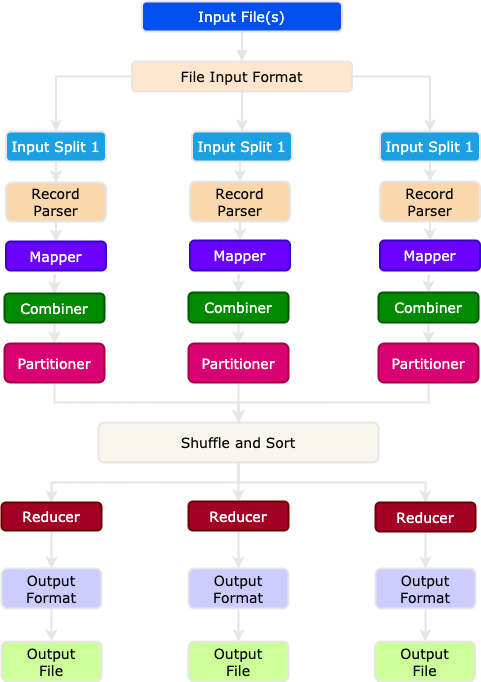
\includegraphics[height=.925\textheight]{./Figures/chapter-02/Map-Reduce.png}
		\caption{Map Reduce Stages } \label{fig:MRSteps}
	\end{figure}			
\end{frame}
%%%%%%%%%%%%%%%%%%%%%%%%%%%%%%%%%%%%%%%%%%%%%%%%%%%%%%
\begin{frame}
	
	\begin{figure}
		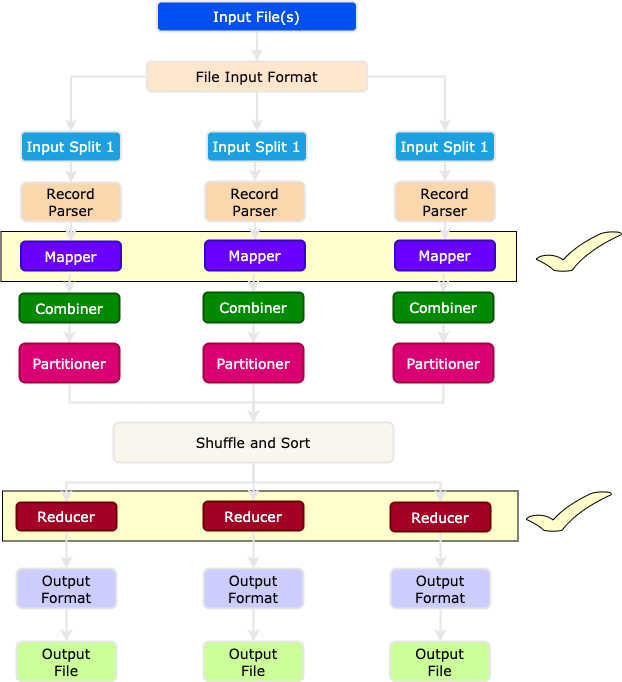
\includegraphics[height=.925\textheight]{./Figures/chapter-02/Map-Reduce_2.png}
		\caption{Map Reduce Stages } \label{fig:MRSteps2}
	\end{figure}			
\end{frame}
%%%%%%%%%%%%%%%%%%%%%%%%%%%%%%%%%%%%%%%%%%%%%%%%%%%%%%
\begin{frame}
	
	\begin{figure}
		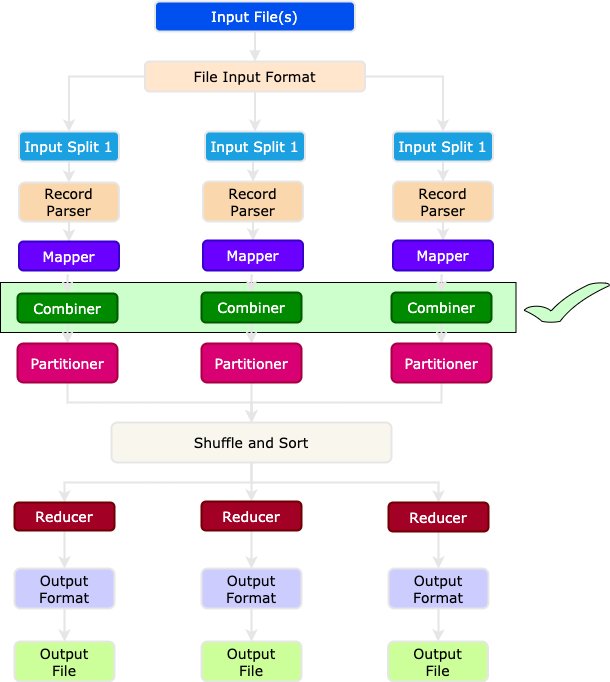
\includegraphics[height=.925\textheight]{./Figures/chapter-02/Map-Reduce-components-combiner.png}
		\caption{Map Reduce Stages } \label{fig:MRSteps2}
	\end{figure}			
\end{frame}

%%%%%%%%%%%%%%%%%%%%%%%%%%%%%%%%%%%%%%%%%%%%%%%%%%%%%%
\begin{frame}[c]{ }
	\frametitle{ The Combiners}
	\centering     
	
	\textcolor{offgreen}{ \large Increase The Map-Reduce Processing Using The Combiners}
\end{frame}
%%%%%%%%%%%%%%%%%%%%%%%%%%%%%%%%%%%%%%%%%%%%%%%%%%%%%%
\begin{frame}
	
	\begin{figure}
		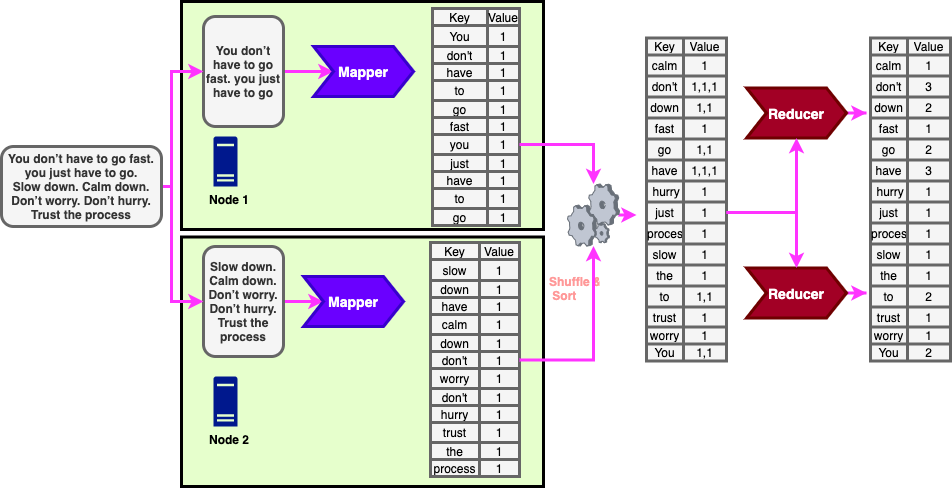
\includegraphics[height=.85\textheight]{./Figures/chapter-02/map-reduce-combiner-ex-1.png}
		\caption{Map Reduce Without Combiner } \label{fig:MRCombiner1}
	\end{figure}			
\end{frame}
%%%%%%%%%%%%%%%%%%%%%%%%%%%%%%%%%%%%%%%%%%%%%%%%%%%%%%
\begin{frame}
	
	\begin{figure}
		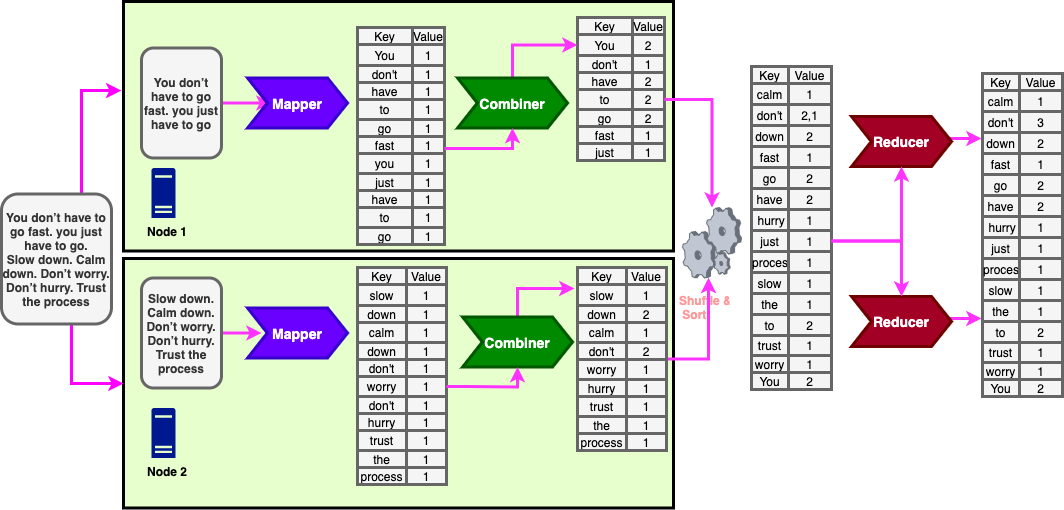
\includegraphics[height=.85\textheight]{./Figures/chapter-02/map-reduce-combiner-ex-2.png}
		\caption{Map Reduce Without Combiner } \label{fig:MRCombiner2}
	\end{figure}			
\end{frame}


%%%%%%%%%%%%%%%%%%%%%%%%%%%%%%%%%%%%%%%%%%%%%%%%%%%%%%%
%\subsection{Further Readings and Assignment}
%
%%%%%%%%%%%%%%%%%%%%%%%%%%%%%%%%%%%%%%%%%%%%%%%%%%%%%%%%%%%%%%%%%%%%%%%%%%%%
%%%% Local Variables:
%%%% mode: latex
%%%% TeX-master: "../main"
%% !TeX root = ../main.tex
%%%% TeX-engine: xetex
%%%% End:
% use no footline.
\begin{frame}[plain, noframenumbering]{Outline}
	\tableofcontents
\end{frame}
%%%%%%%%%%%%%%%%%%%%%%%%%%%%%%%%%%%%%%%%%%%%%%%%%%%%%%
\section{Hadoop and Map-Reduce}


\begin{frame}
\frametitle{Chapter Objectives}

\begin{itemize}
	\item<1-> Introduction to Hadoop and its echo-systems. \pause
	\item<2-> Why we need Hadoop? \pause
	\item<3-> Understand the concept of HDFS and Map-Reduce.
	\item<4-> Developing Map-Reduce applications. \pause
	\item<5-> Using HiveQL over Map-Reduce. \pause
	\item<6-> Hadoop advantages and disadvantages with use cases? \pause
\end{itemize}

\end{frame}

%%%%%%%%%%%%%%%%%%%%%%%%%%%%%%%%%%%%%%%%%%%%%%%%%%%%%%

\subsection{Hadoop Architecture}
\begin{frame}
\frametitle{\subsecname}
\begin{itemize} 
	\item Any Big Data solution working based distributed systems.
	\item What is distributed systems in brief?
\end{itemize}
\end{frame}

%%%%%%%%%%%%%%%%%%%%%%%%%%%%%%%%%%%%%%%%%%%%%%%%%%%%%%


\subsubsection{Storage}
\begin{frame}
\frametitle{Storage}
\begin{itemize} 
	\item Any Big Data solution working based distributed systems.
	\item What is distributed systems in brief?
\end{itemize}
\end{frame}

%%%%%%%%%%%%%%%%%%%%%%%%%%%%%%%%%%%%%%%%%%%%%%%%%%%%%%

\subsubsection{YARN}
\begin{frame}
\frametitle{YARN}
\begin{itemize} 
	\item Any Big Data solution working based distributed systems.
	\item What is distributed systems in brief?
\end{itemize}
\end{frame}

%%%%%%%%%%%%%%%%%%%%%%%%%%%%%%%%%%%%%%%%%%%%%%%%%%%%%%

\subsubsection{Hadoop I/O}
\begin{frame}
\frametitle{Hadoop I/O}
\begin{itemize} 
	\item Any Big Data solution working based distributed systems.
	\item What is distributed systems in brief?
\end{itemize}
\end{frame}

%%%%%%%%%%%%%%%%%%%%%%%%%%%%%%%%%%%%%%%%%%%%%%%%%%%%%%

\subsubsection{Processing}
\begin{frame}
\frametitle{Processing}
\begin{itemize} 
	\item Any Big Data solution working based distributed systems.
	\item What is distributed systems in brief?
\end{itemize}
\end{frame}

%%%%%%%%%%%%%%%%%%%%%%%%%%%%%%%%%%%%%%%%%%%%%%%%%%%%%%

\subsection{Map-Reduce}
\begin{frame}
\frametitle{\subsecname}
\begin{itemize} 
	\item Any Big Data solution working based distributed systems.
	\item What is distributed systems in brief?
\end{itemize}
\end{frame}

%%%%%%%%%%%%%%%%%%%%%%%%%%%%%%%%%%%%%%%%%%%%%%%%%%%%%%

\subsubsection{Map-Reduce Components}
\begin{frame}
\frametitle{Map-Reduce Components}
\begin{itemize} 
	\item Any Big Data solution working based distributed systems.
	\item What is distributed systems in brief?
\end{itemize}
\end{frame}

%%%%%%%%%%%%%%%%%%%%%%%%%%%%%%%%%%%%%%%%%%%%%%%%%%%%%%

\subsubsection{Word-Count Example}
\begin{frame}
\frametitle{Word-Count Example}
\begin{itemize} 
	\item Any Big Data solution working based distributed systems.
	\item What is distributed systems in brief?
\end{itemize}
\end{frame}

%%%%%%%%%%%%%%%%%%%%%%%%%%%%%%%%%%%%%%%%%%%%%%%%%%%%%%

\subsection{Pig}
\begin{frame}
\frametitle{Pig}
\begin{itemize} 
	\item Any Big Data solution working based distributed systems.
	\item What is distributed systems in brief?
\end{itemize}
\end{frame}

%%%%%%%%%%%%%%%%%%%%%%%%%%%%%%%%%%%%%%%%%%%%%%%%%%%%%%

\subsection{Hive}
\begin{frame}
\frametitle{Hive}
\begin{itemize} 
	\item Any Big Data solution working based distributed systems.
	\item What is distributed systems in brief?
\end{itemize}
\end{frame}


%%%%%%%%%%%%%%%%%%%%%%%%%%%%%%%%%%%%%%%%%%%%%%%%%%%%%%

\subsection{ZooKeeper}
\begin{frame}
\frametitle{ZooKeeper}
\begin{itemize} 
	\item Any Big Data solution working based distributed systems.
	\item What is distributed systems in brief?
\end{itemize}
\end{frame}

\subsection{Further Readings and Assignment}


%%%%%%%%%%%%%%%%%%%%%%%%%%%%%%%%%%%%%%%%%%%%%%%%%%%%%%%%%%%%%%%%%%%%%%%%%%%
%%% Local Variables:
%%% mode: latex
%%% TeX-master: "../main"
% !TeX root = ../main.tex
%%% TeX-engine: xetex
%%% End:
%    \include{Ch04-Spark/FN-Scala}
%    \include{Ch04-Spark/Spark}
%    \include{Ch05-BigData-Applications/Applications}
%    \include{Ch06-Massaging-Systems/Massaging-Systems}
%    \include{Ch07-DataOrchestration/Orchestration}
%    \include{Ch08-NoSqlDB/NoSql}
%    \include{Ch09-Elastic/Elastic}
%    \include{Ch10-Architecture/Architecture}
%    \include{Appendix/Appendix}
%%%%%%%%%%%%%%%%%%%%%%%%%%%%%%%%%%%%%%%%%%%%%%%%%%%%%%

\begin{frame}[c]{ }
    \centering     
   
    \textcolor{offgreen}{ \large Thank you for watching!}
\end{frame}


\begin{frame}[c]{ }
    \centering 
    \textcolor{offyellow}{\large See you in the next video \Smiley{}}
\end{frame}
    %%%%%%%%%%%%%%%%%%%%%%%%%%%%%%%%%%%%%%%%%%%%%%%%%%%%%%%%%%%%%%%%%%%%%%%%%%%%%%%%%%%%%%%
\end{document}

%%% Local Variables:
%%% mode: latex
%%% TeX-master: t
%%% TeX-engine: xetex
%%% End:
